\documentclass[12pt]{article}   % use documentclass amsart too if you want
\usepackage{amsmath,amsthm,amssymb}
\usepackage[margin=1in]{geometry}
\usepackage{color}
\usepackage{hyperref}
\usepackage{graphicx}
\usepackage{fancyhdr} % COMMENT THIS OUT TO TURN OFF FANCY HEADERS
\usepackage{verbatim}
\usepackage{setspace}

\hypersetup{
  colorlinks= true, %Colours links instead of ugly boxes
  urlcolor   = blue, %Colour for external hyperlinks
  linkcolor  = blue, %Colour of internal links
  citecolor  = blue %Colour of citations
}





\newtheorem{theorem}[equation]{Theorem}
\newtheorem{lemma}[equation]{Lemma}
\newtheorem{corollary}[equation]{Corollary}
\theoremstyle{definition}
\newtheorem{exercise}[equation]{Exercise}

\newtheorem{example}[equation]{Example}
\newtheorem{definition}[equation]{Definition}
\newtheorem{question}[equation]{Question}
\newtheorem{remark}[equation]{Remark}

\numberwithin{equation}{section}

%@@@@@@@@@@@@@@@@@@@@@@@@@@@@@@@@@@@@@@@@@@@@@@@@@@@@@@@@@@@@@@@@@@@@@@@@@@@@@@@@@@@@@@@@@

\begin{document}
\parskip10pt
\parindent0pt
\baselineskip15pt
\doublespacing

\title{APPM 2350 Project 2: Hiking}
\author{Davis Landry (section 223), Mahalie Hill (section 223)\\Mia Miller (section 213) \\ Jonathan Kish, Maribeth Oscamou}

%I think we should add a photo here for the cover page
\pagestyle{fancy}
\renewcommand{\sectionmark}[1]{\markright{#1}{}}

\fancyhf{}

\rhead{\fancyplain{}{\thepage}} % predefined ()
\lhead{\fancyplain{}{\rightmark }} % 1. sectionname, 1.1 subsection name etc
%\cfoot{\fancyplain{}{\thepage}}

\maketitle
\begin{figure} [h]
  \centering
  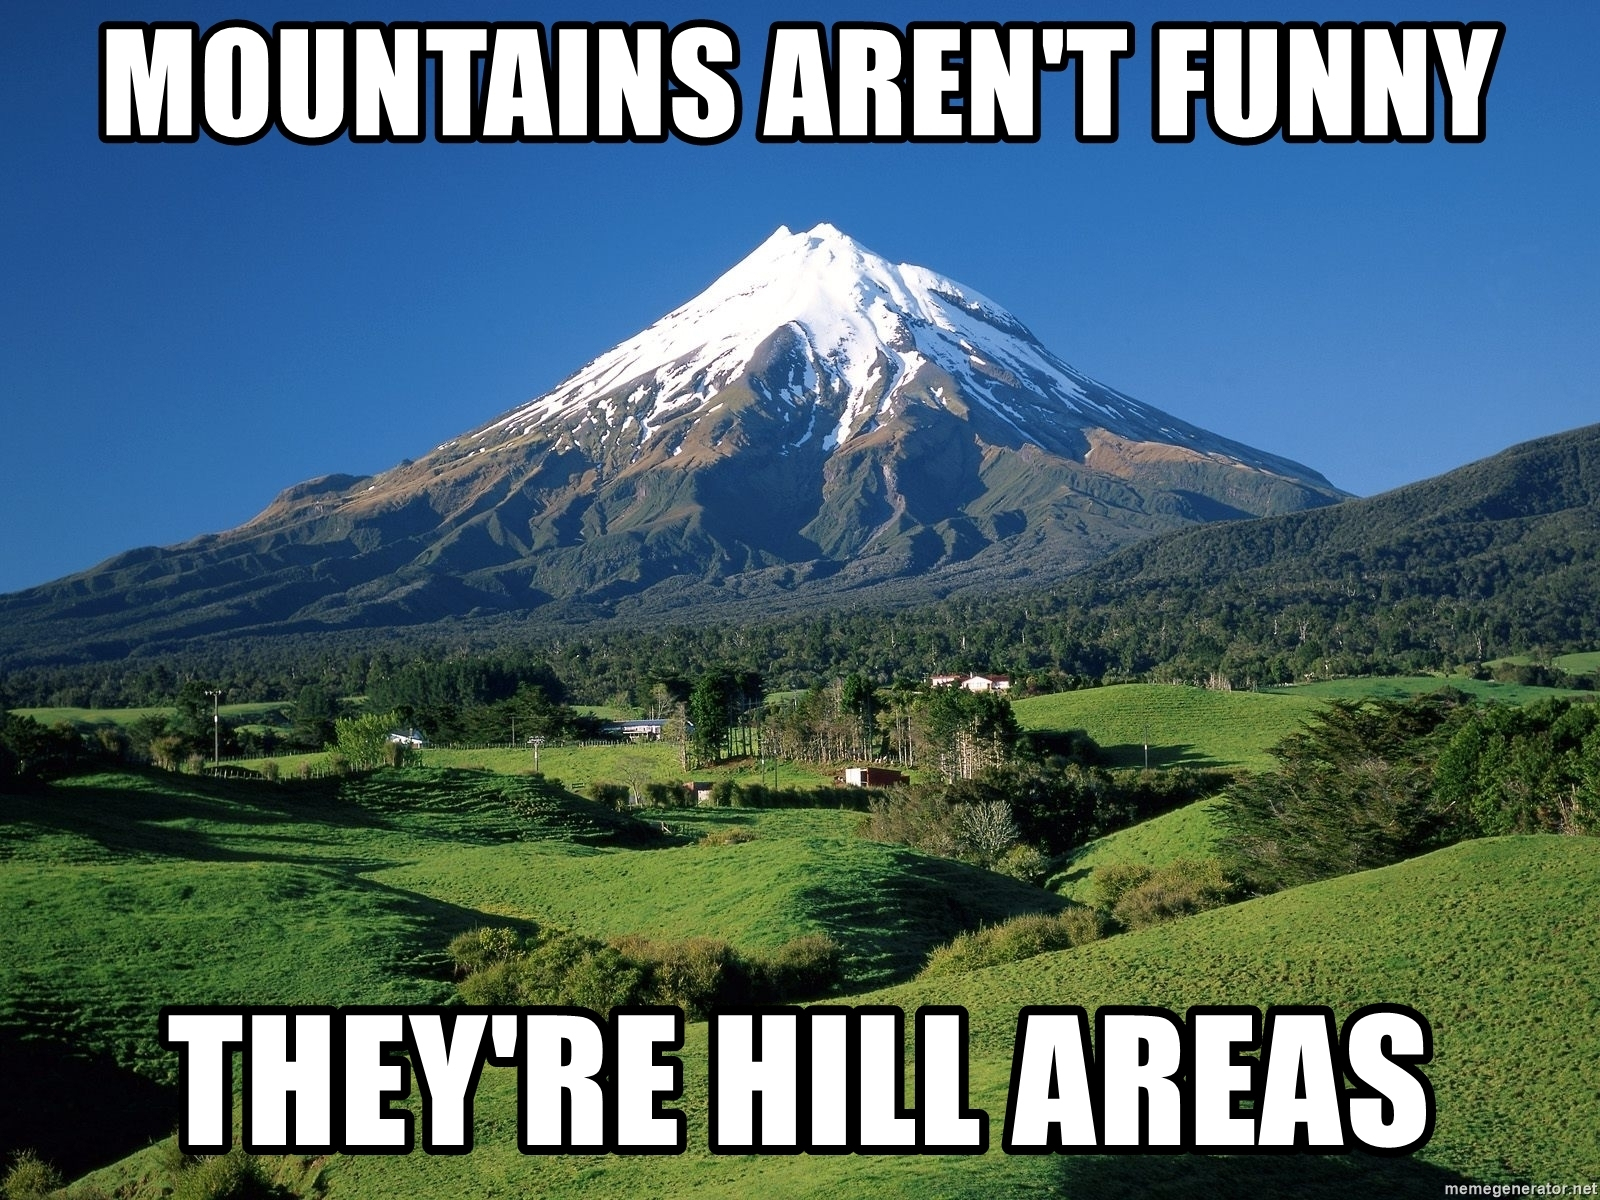
\includegraphics[width=13cm]{../images/mountains-arent-funny-theyre-hill-areas.jpg}
  \label{fig:coverPage}
\end{figure}

\newpage
%\setcounter{page}{2}
\tableofcontents
\newpage
%@@@@@@@@@@@@@@@@@@@@@@@@@@@@@@@@@@@@@@@@@@@@@@@@@@@@@@@@@@@@@@@@@@@@@@@@@@@@@@@@@@@@@@@@@
\newpage
\lhead{Landry, Hill, Miller Project 2}
%\setcounter{page}{2}

\section{Introduction} \label{APPM2350proj01sec01}

\quad Welcome to Colorado! Before we embark on this epic journey through the Lagrange Mountain range, we have compiled a travel packet for you to understand the trail system we will be hiking. We promise, after reading this trail analysis, you'll feel equiped to conquer this trail.
\newpage
%@@@@@@@@@@@@@@@@@@@@@@@@@@@@@@@@@@@@@@@@@@@@@@@@@@@@@@@@@@@@@@@@@@@@@@@@@@@@@@@@@@@@@@@@
%\setcounter{page}{4}
\section{Basic Trail Information} \label{APPM2350proj01sec02}

\quad The Lagrange loop is located a short drive from Boulder, CO. It is a 2.24$mi$ hike, with 6033$ft$ of elevation change. You better be in great shape, because we expect to finish this hike in roughly 1 hour 34 minutes. The hike consists of jaw-dropping views of Lake Mochi, with views of the sheer sides of Mount Adamore in the background. This trail is primarily used for speed hiking and trail running because the Honey Badger at Curtis Pass enjoys giving chase to trail users, a great endurance training regime for the super athletes of Colorado. Dogs are not allowed due to the Honey Badger, so leave your furry friends at home.
\newpage
%@@@@@@@@@@@@@@@@@@@@@@@@@@@@@@@@@@@@@@@@@@@@@@@@@@@@@@@@@@@@@@@@@@@@@@@@@@@@@@@@@@@@@@@@@@@@@@@@@@@@@@@@@@@@@@@@@@@@@@
%\setcounter{page}{7}
\section{The Specs}
\label{APPM2350proj01sec03}

\begin{figure} [h]
  \centering
  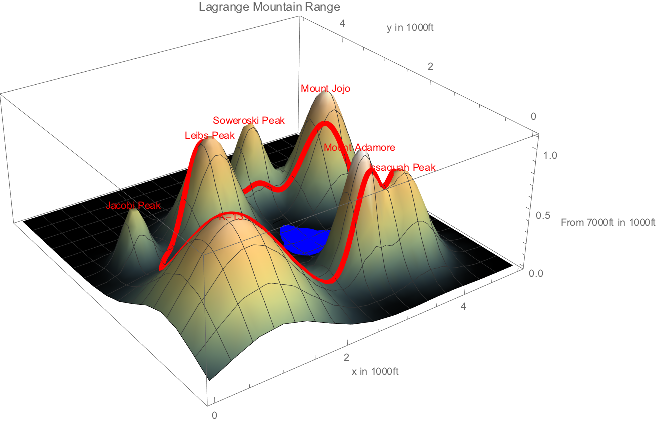
\includegraphics[width=10cm]{../images/lakeCorrect.png}
  \caption{Lagrange Mountain Range with Selected Trail}
  \label{fig:7humpswithtrail}
\end{figure}

\quad Pictured in \autoref{fig:7humpswithtrail}, you can see the general trail outline. The trail is a two-way path, so it can be taken from either direction from the trailhead. It is highly recommended that those with bad knees go counterclockwise around the loop, due to the steep section of trail on Mount Adamore.

\begin{figure} [h]
  \centering
  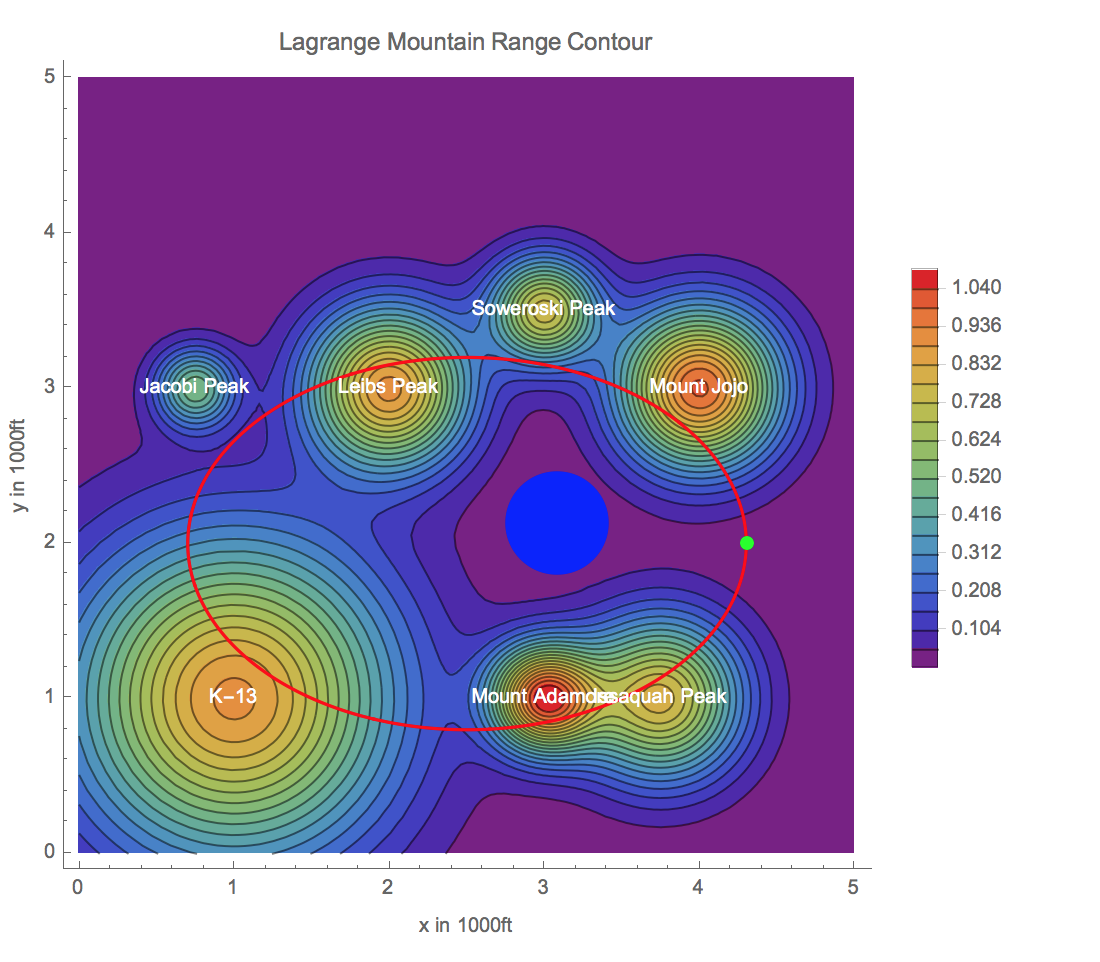
\includegraphics[width=12cm]{../images/topoLake.png}
  \caption{Lake Mochi in the Topographical Map}
  \label{fig:lakeMochiTopo}
\end{figure}
%\begin{figure} [h]
%  \centering
%  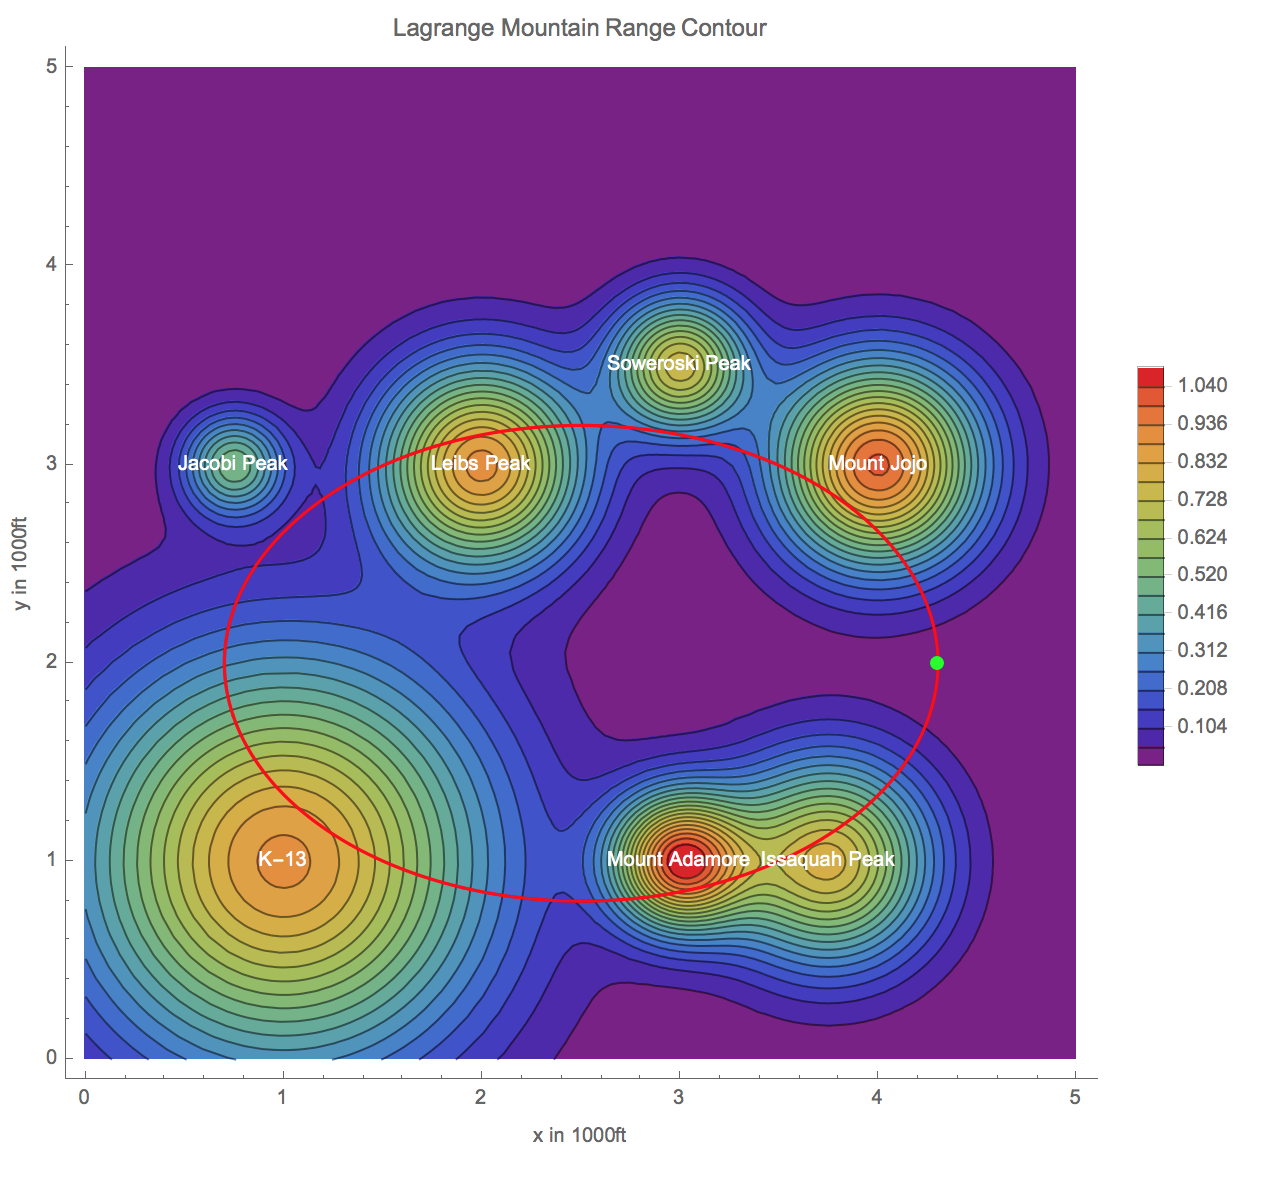
\includegraphics[width=10cm]{../images/topoMtnCorrect.png}
%  \caption{Topographical Map for Lagrange Mountain Range}
%  \label{fig:topoOne}
%\end{figure}
\begin{figure} [h]
  \centering
  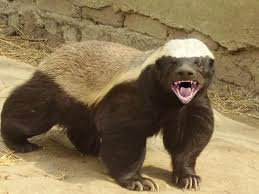
\includegraphics[width=10cm]{../images/honey_badger.jpeg}
  \caption{Real Life Sighting of Honey Badger}
  \label{fig:honeyB}
\end{figure}

\newpage

\quad Looking at \autoref{fig:lakeMochiTopo}, the general steepness of the trail can be assumed. Note that at Curtis pass, the trail travels uphill. This is where our friend the Honey Badger lives, and he despises the frequent visitors on his doorstep. Beware, because we will have to pick up our pace through here to avoid him. The trail slope is fairly steep, at a $60.5\%$ grade, and the rate of elevation change is $2.9ft/hr$. Hopefully those sea level lungs of you out-of-staters can handle the stress.



\quad The steepest section of trail along the Lagrange Loop is 73 minutes into the hike, so make sure to save water and snacks for this section. The most leisurely section of the hike, with the smallest elevation change around 31 minutes into the hike.
\quad Although that is our steepest climb, and flattest section, the trail is highly variable, so we will be embarking on a number of climbs throughout. If you are wondering where those other climbs are in relation to the time we will spend out hiking, take a look at \autoref{fig:changeEl}, so you know how many snacks and how much water to save. Hydrate or die folks!

\begin{figure} [h]
  \centering
  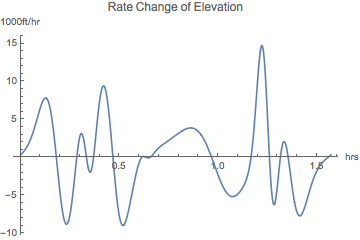
\includegraphics[width=10cm]{../images/changeEl.png}
  \caption{Rate of Change for Elevation Throughout the Trail}
  \label{fig:changeEl}
\end{figure}

\quad Mount Adamore is the highest peak in the Lagrange Range, with an elevation of 8,100.8$ft$. The path does not go to the peak, so the maximum elevation we will reach $7,934ft$, easily accomplishable with lungs acclimated to lower elevations. No altitude sickness today kids! We will be staying well under $9,000ft$.




%\begin{figure} [h]
%  \centering
%  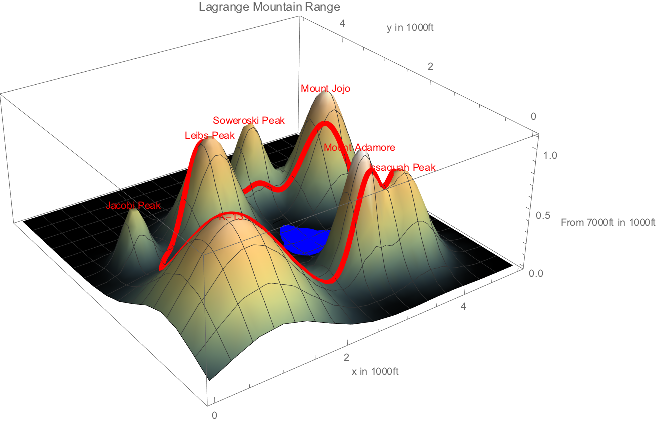
\includegraphics[width=12cm]{../images/lakeCorrect.png}
%  \caption{Lake Mochi in the Lagrange Mountain Range}
  %\label{fig:lakeMochi}
%\end{figure}

\quad \autoref{fig:lakeMochiTopo} Nothing is more of a mountain adventure than swimming in an alpine lake! Lake Mochi sits in the valley created by the Lagrange Range, a pristine oasis surrounded by beautiful mountains. Note that the trail does not go directly to the lake, but a little bit of bush-wacking from the trailhead can get us there in a few minutes without too much elevation change. View \autoref{fig:lakeMochiTopo} to get a sense of how far it is to the lake based on the length of the rest of the hike.

\newpage
%@@@@@@@@@@@@@@@@@@@@@@@@@@@@@@@@@@@@@@@@@@@@@@@@@@@@@@@@@@@@@@@@@@@@@@@@@@@@@@@@@@@@@@@@
%\setcounter{page}{12}
\section{Trail Lore} \label{APPM2350proj02sec05}

\quad These beautiful peaks encase a whole lot of rock. Actually, about $4.94*10^{10}ft^3$, to be more precise if we consider the trail and the valley the trail surrounds. For the rock above $7,000ft$, there is a legend that Clairautnium can be found in scarce quantities. Roughly $2.5ng$ of Clairautnium is estimated to be encased in the entire mountain range. With that being said, coming across any on our hike is highly unlikely. Even if a "nugget" held all of the Clairautnium in the entire range, it would probably not be visible to the human eye. A specific speck of dust on a sandy trail is hard to spot.

\quad Why would people care about Clairautnium you ask? Well legend has it that the Clairautnium has a unique ability where once touched, you will actually be transported to the land of Leibniz Mountain Range, where the peaks are ever changing with time. Here, some of the finest gems can be found due to the malleability of the soil. However, any visitors must work quickly to find what they are looking for as the range changes with every hour and it completely unpredictable. Now I know this hike is already a challenge for an out-of-stater but it becomes incredibly worth it for the chance we have of riches and adrenaline rushing adventure. Although it may be hard for us to find Clairautnium, the search could be worth it.
\newpage
%@@@@@@@@@@@@@@@@@@@@@@@@@@@@@@@@@@@@@@@@@@@@@@@@@@@@@@@@@@@@@@@@@@@@@@@@@@@@@@@@@@@@@@@@
%\setcounter{page}{13}
\section{Summary} \label{APPM2350proj02sec06}

\quad Hopefully you are intrigued enough to come adventure throughout the Lagrange Range. Remember to pack enough snacks and water to maintain high morale and energy! Hungry friends are not happy friends... So make sure to bring a little extra for the Honey Badger. At the speed recommended to conquer this trail, hopefully you have been training for the steep climbs. Let's get into the Colorado mindset and take on the trails!
\newpage
%@@@@@@@@@@@@@@@@@@@@@@@@@@@@@@@@@@@@@@@@@@@@@@@@@@@@@@@@@@@@@@@@@@@@@@@@@@@@@@@@@@@@@@@@
%\setcounter{page}{14}
\section{Lagrange Loop Not Challenging Enough?} \label{APPM2350proj02sec07}

\quad  Now, if we are looking for a greater challenge we need to know more about the Leibniz Mountain Range. Sometimes the peaks can be very drastic slopes as well as some being minimal and more hill shaped. Below are a few instances that high tech instruments have been able to capture before for a sample of what the layout could be if we can get in. The trail may require more of a bushwhacking approach over the previous plan because there is no constant trail. Along with these three past instances, there was a study done where 50 straight hours of the mountain range layout were able to be recorded which can be found in the end of this paper if you are still unsure about the possible terrain we will encounter.

\begin{figure} [h]
  \centering
  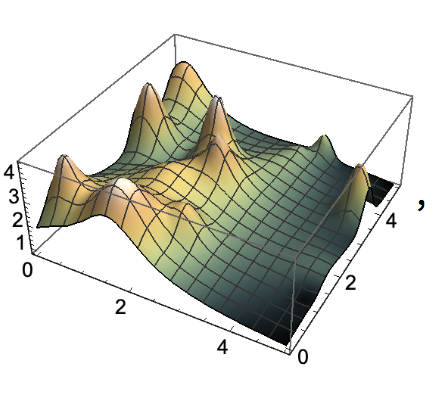
\includegraphics[width=10cm]{../images/mtn1.png}
  \caption{A Previous Mountain Range Layout}
\end{figure}

\begin{figure} [h]
  \centering
  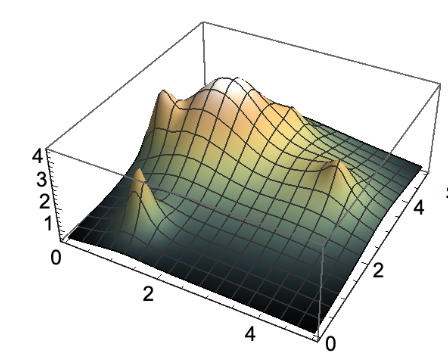
\includegraphics[width=10cm]{../images/mtn2.png}
  \caption{A Previous Mountain Range Layout}
\end{figure}

\begin{figure} [h]
  \centering
  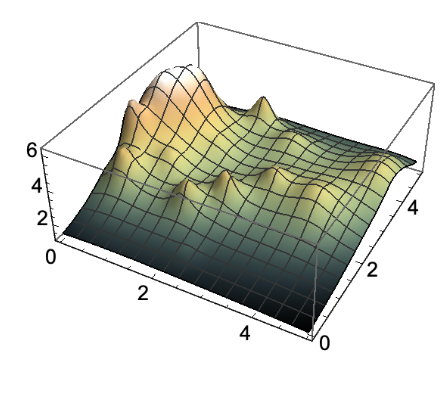
\includegraphics[width=10cm]{../images/mtn3.png}
  \caption{A Previous Mountain Range Layout}
\end{figure}
\newpage
%@@@@@@@@@@@@@@@@@@@@@@@@@@@@@@@@@@@@@@@@@@@@@@@@@@@@@@@@@@@@@@@@@@@@@@@@@@@@@@@@@@@@@@@@
%\setcounter{page}{15}
\section{Appendix} \label{APPM2350proj02sec08}


%@@@@@@@@@@@@@@@@@@@@@@@@@@@@@@@@@@@@@@@@@@@@@@@@@@@@@@@@@@@@@@@@@@@@@@@@@@@@@@@@@@@@@@@@


\end{document}
